\documentclass[11pt,a4paper]{article}

\usepackage[utf8]{inputenc}
\usepackage[T1]{fontenc}
\usepackage{lmodern}
\usepackage[margin=0.82in]{geometry}
\usepackage[table]{xcolor}
\usepackage{array}
\usepackage{tabularx}
\usepackage{booktabs}
\usepackage{enumitem}
\usepackage{titlesec}
\usepackage{fancyhdr}
\usepackage{lastpage}
\usepackage{hyperref}
\usepackage{tikz}

\definecolor{TextInk}{HTML}{233142}
\definecolor{HeadingBlue}{HTML}{1D3557}
\definecolor{AccentTeal}{HTML}{2A7F92}
\definecolor{AccentGold}{HTML}{C58B4E}
\definecolor{RuleGray}{HTML}{D6E0E5}
\definecolor{TableStripe}{HTML}{F3F8FA}
\definecolor{SoftTint}{HTML}{F7F4EE}
\definecolor{SoftBlue}{HTML}{EEF6F8}
\definecolor{SoftGreen}{HTML}{EEF7F0}
\definecolor{SoftRed}{HTML}{FBF0EF}

\hypersetup{
  colorlinks=true,
  linkcolor=HeadingBlue,
  urlcolor=AccentTeal,
  pdftitle={IB Geography SL Study Pack - 2026-04-27},
  pdfauthor={IB Geography SL Preparation}
}

\color{TextInk}
\setlength{\parskip}{0.52em}
\setlength{\parindent}{0pt}
\setlength{\tabcolsep}{6pt}
\renewcommand{\arraystretch}{1.22}
\setlist[itemize]{leftmargin=1.35em,itemsep=3pt,topsep=4pt}
\setlist[enumerate]{leftmargin=1.5em,itemsep=3pt,topsep=4pt}

\newcolumntype{Y}{>{\raggedright\arraybackslash}X}
\newcolumntype{L}[1]{>{\raggedright\arraybackslash}p{#1}}

\titleformat{\section}
  {\normalfont\huge\sffamily\bfseries\color{HeadingBlue}}
  {}{0pt}{}
  [\vspace{0.15em}{\color{AccentGold}\titlerule[1pt]}]

\titleformat{\subsection}
  {\normalfont\Large\sffamily\bfseries\color{AccentTeal}}
  {}{0pt}{}

\titleformat{\subsubsection}
  {\normalfont\large\sffamily\bfseries\color{HeadingBlue}}
  {}{0pt}{}

\titlespacing*{\section}{0pt}{1.4em}{0.65em}
\titlespacing*{\subsection}{0pt}{1.0em}{0.35em}
\titlespacing*{\subsubsection}{0pt}{0.8em}{0.25em}

\pagestyle{fancy}
\setlength{\headheight}{14pt}
\fancyhf{}
\fancyhead[L]{\sffamily\color{AccentTeal}Mon 2026-04-27}
\fancyhead[R]{\sffamily\color{HeadingBlue}IB Geography SL}
\fancyfoot[C]{\sffamily\color{HeadingBlue}\thepage\ of \pageref{LastPage}}
\renewcommand{\headrulewidth}{0.4pt}
\renewcommand{\footrulewidth}{0pt}

\newcommand{\term}[1]{\textcolor{HeadingBlue}{\textbf{#1}}}
\newcommand{\exam}[1]{\textcolor{AccentTeal}{\textbf{#1}}}
\newcommand{\boxnote}[3]{%
\noindent\colorbox{#1}{%
  \begin{minipage}{0.965\textwidth}
  \sffamily
  \textbf{\textcolor{HeadingBlue}{#2}} #3
  \end{minipage}
}}

\begin{document}

\begin{center}
  {\sffamily\bfseries\color{HeadingBlue}\LARGE IB Geography SL Study Pack}\\[0.25em]
  {\sffamily\bfseries\color{AccentTeal}\Large Monday 2026-04-27}\\[0.35em]
  {\sffamily\color{TextInk}Urban Processes, Patterns, Causes + Global Climate Vulnerability And Resilience}
\end{center}

\vspace{0.5em}

\boxnote{SoftBlue}{How this pack follows the plan.}{The April 27 schedule is a
weekday session: \term{Audio 1} covers Urban environments processes, patterns,
and causes, especially \term{urbanization}, \term{centripetal and centrifugal
movements}, and \term{infrastructure growth}. \term{Audio 2} covers
\term{Global climate - vulnerability and resilience}, especially causes and
major consequences. The \term{25 minute} practice block asks for one
\exam{explain} paragraph and one \exam{analyse} paragraph; use the separate
April 27 workbook for that writing practice.}

\section{Today's Target}

By the end of this session, you should be able to:

\begin{itemize}
  \item explain how urbanization changes city size, land use, housing demand,
  services, and infrastructure
  \item distinguish \term{centripetal movement} from \term{centrifugal
  movement} in an urban system
  \item connect urban growth to infrastructure demand in transport, housing,
  water, sanitation, energy, and communications
  \item explain the enhanced greenhouse effect and the main human drivers of
  climate change
  \item describe major climate consequences for food, water, health, and
  settlements
  \item connect climate consequences to ecosystems and economies
  \item use \term{vulnerability} and \term{resilience} accurately in a Paper 2
  paragraph
  \item write one concise \exam{explain} paragraph and one more relational
  \exam{analyse} paragraph
\end{itemize}

\subsection{Session Structure}

\rowcolors{2}{TableStripe}{white}
\begin{tabularx}{\textwidth}{L{0.18\textwidth}Y L{0.22\textwidth}}
\toprule
\textbf{Block} & \textbf{Focus} & \textbf{Output} \\
\midrule
Audio 1 & Urbanization, centripetal and centrifugal movement, infrastructure
growth & Urban process chain \\
Audio 2 & Climate causes, consequences, vulnerability, and resilience & Climate
risk chain \\
25 min practice & One explain paragraph and one analyse paragraph & Two marked
paragraphs in the workbook \\
\bottomrule
\end{tabularx}
\rowcolors{2}{}{}

\boxnote{SoftTint}{Carry-forward from April 25.}{Before Audio 1, look at the
weakest Urban environments item from the April 25 workbook. Try to include that
weak point in today's urban process chain, especially if it involved
urbanization, migration, infrastructure, or evaluation.}

\section{Audio 1 Script}
\subsection{Urban Processes, Patterns, Causes, And Infrastructure Growth}

\textit{Target length: about 12 minutes at a natural revision pace. Pause after
each numbered process chain and say the chain aloud from memory.}

Monday, 2026-04-27. Audio 1. \textbf{Minute 0--2: key terms.}
Today returns to \term{Urban environments}, but with a narrower target than
Friday's overview or Saturday's depth practice. The focus is process, pattern,
and cause. In other words, what is moving, what spatial pattern appears, and why
does that pattern form? The key words are \term{urbanization},
\term{centripetal movement}, \term{centrifugal movement}, and
\term{infrastructure growth}.

\term{Urbanization} means an increasing proportion of a population living in
urban areas. It can happen through rural-to-urban migration, natural increase
within cities, expansion of urban boundaries, or reclassification of settlements
as urban. It is not just a bigger city on a map. It changes land value, housing
demand, transport flows, employment structure, waste production, water demand,
energy demand, and the political importance of urban planning. A strong answer
therefore treats urbanization as a process that creates linked consequences.

\term{Centripetal movement} means movement toward a center or concentration of
activity. In urban geography, it can describe people, investment, services, or
economic functions being pulled into a city or a central district. Common pulls
include jobs, education, healthcare, safety, transport nodes, social networks,
entertainment, finance, universities, specialist services, and the prestige of a
central location. When centripetal forces are strong, a city may densify,
central land values may rise, and pressure on transport, housing, and public
services may increase.

\term{Centrifugal movement} means movement away from a center. In cities, it can
describe people, industries, offices, retail, or services shifting outward to
suburbs, edge cities, logistics parks, or the rural-urban fringe. Push factors
can include high land values, congestion, pollution, lack of space, older
buildings, crime fears, weak parking, and conflict over land use. Pull factors
outside the center can include cheaper land, larger homes, road access,
greenfield sites, business parks, and a perceived better quality of life. This
outward movement can create suburbanization, sprawl, longer commuting, land
consumption, and new infrastructure needs.

\textbf{Minute 2--5: urbanization as a process chain.}
Use a process chain when you explain urbanization. The simplest version is:
\term{rural and urban causes} $\rightarrow$ \term{migration or natural increase}
$\rightarrow$ \term{urban population growth} $\rightarrow$ \term{demand for land,
housing, jobs, transport, and services} $\rightarrow$ \term{social and
environmental consequences}. That chain is more useful than a definition because
it can become a paragraph under exam pressure.

Start with causes. Rural push factors can include low farm income, land
shortage, mechanization, drought, conflict, poor services, or limited education
and healthcare. Urban pull factors can include formal and informal employment,
higher wages, schools, hospitals, social networks, safety, markets, and the
hope of social mobility. Natural increase inside cities matters too,
especially where migrants are young and birth rates remain relatively high.
Cities can therefore grow even if migration slows.

Now connect cause to pattern. Rapid urbanization often produces outward
expansion at the edge, densification near job centers, informal settlement where
formal housing is unaffordable, and rising competition for accessible land. A
wealthier city may show growth through apartment construction, transport-linked
density, and suburban expansion. A lower-income or very rapidly growing city may
show greater pressure through overcrowding, informal housing, weak sanitation,
and transport overload. Do not write as if every city grows in the same way.
Pattern depends on income, governance, land ownership, transport, planning
capacity, and physical geography.

Infrastructure is the bridge between growth and impact. \term{Infrastructure}
means the basic physical and organizational systems that allow a city to
function. It includes transport networks, roads, rail, buses, water supply,
sanitation, drainage, waste collection, electricity, internet, schools,
healthcare, housing, ports, airports, and emergency services. Urbanization
raises demand for all of these. When infrastructure grows more slowly than
population, stress appears: congestion, unreliable water, poor sanitation,
overcrowded schools, informal power connections, flood risk from weak drainage,
and long commuting times.

\textbf{Minute 5--7: centripetal and centrifugal movement.}
Centripetal and centrifugal movement help you explain why urban systems are
dynamic rather than fixed. A central business district can attract firms
because it has accessibility, face-to-face contact, specialist labor, financial
services, transport links, and high visibility. Those are centripetal forces.
However, the same central area may repel some households or businesses because
land is expensive, roads are congested, buildings are older, and space is
limited. Those are centrifugal forces. A single district can therefore pull in
some activities while pushing out others.

Suburbanization is a classic centrifugal process. Households may move outward
because they want more space, cheaper housing, gardens, schools, or lower
perceived crime. Businesses may move outward because they want cheaper land,
larger sites, road access, parking, and logistics space. The pattern can include
lower-density housing, retail parks, edge offices, industrial estates, and
longer commutes. The evaluation is important: suburbanization may improve living
space for some groups, but it can consume farmland, increase car dependence,
raise emissions, and leave poorer households with weaker access if public
transport is limited.

Reurbanization and gentrification can be centripetal processes. Investment and
higher-income residents may return to inner districts because of cultural
amenities, short commutes, historic buildings, universities, waterfront
redevelopment, or public investment. In Detroit, the case-study anchor from your
student sheet, this can be linked to selective reinvestment after long-term
industrial decline and population loss. The careful argument is that
reinvestment can improve buildings, services, image, and employment in selected
districts, but it may also raise rents or concentrate benefits among developers,
new residents, and visitors. The process is not just physical; it changes who
can afford to stay in the place.

\textbf{Minute 7--9: infrastructure growth and uneven access.}
Infrastructure growth can be planned, market-led, reactive, or informal. A
planned transport extension can open land for housing and employment. A private
housing development can create demand for roads, water, schools, and shops. A
rapidly growing informal settlement can build its own small-scale water,
electricity, transport, and retail systems before formal services arrive. A
government can then upgrade services later, ignore the settlement, or clear it.
Each choice creates a different social outcome.

The most important exam idea is that infrastructure access is uneven. A city may
have modern airports, office districts, and expressways while some households
lack reliable water, sanitation, drainage, or affordable transport. This means
urban infrastructure is not only an engineering issue. It is also a question of
equity. Who is connected? Who pays? Which districts are prioritized? Which
groups are exposed to flooding, pollution, or long journeys because
infrastructure is weak?

Use this chain for an \exam{explain} answer: \term{urbanization increases
population and economic activity} $\rightarrow$ \term{demand for transport,
housing, water, sanitation, energy, and services rises} $\rightarrow$ \term{if
investment and planning lag behind, capacity is exceeded} $\rightarrow$
\term{congestion, informal housing, service gaps, and environmental stress
increase}. That is the skeleton of today's explain paragraph.

\textbf{Minute 9--10: named examples and case-study discipline.}
Use your class examples first. The student case-study sheet lists
\term{gentrification in Detroit}. Detroit can help with deindustrialization,
selective reinvestment, gentrification, and social inequality. It is less useful
for every type of urbanization because Detroit is also associated with
population decline and restructuring. If you use it today, use it for movement
within an urban system: industrial activity moved out or declined, investment
returned selectively, and some central districts became more attractive to
capital and higher-income users.

For rapid urbanization and infrastructure pressure, use the exact city your
class has studied if you have one. If your notes include Mumbai, Lagos, Jakarta,
Nairobi, or another rapidly growing city, use that place instead of inventing a
new example. The minimum case-study detail should be: place name, growth
process, infrastructure pressure, affected group, response, and limitation.
Without those details, keep the answer general and mark the case-study gap in
the workbook.

\textbf{Minute 10--12: model command-term paragraph.}
Here is a model \exam{explain} paragraph. Urbanization can create
infrastructure pressure because city population growth increases demand faster
than services can be expanded. Rural-to-urban migration and natural increase add
people who need housing, transport, water, sanitation, electricity, schools, and
healthcare. If city authorities lack money, planning capacity, or land for
formal housing, population growth may produce overcrowding and informal
settlements where drainage, waste collection, and safe water are limited. The
pressure is therefore not caused by population growth alone; it is caused by the
interaction between growth, poverty, land value, and the speed of infrastructure
investment.

Now make the paragraph more analytical. Centripetal and centrifugal movements
can operate at the same time, creating a more uneven city. Central districts may
attract offices, services, tourists, and higher-income residents because of
accessibility and cultural amenities, while lower-income households or
space-hungry industries may be pushed outward by rent, congestion, and land
competition. This means urban growth does not simply spread evenly from the
center. It reshapes the city through selective concentration and dispersal,
producing both renewed inner districts and expanding peripheral zones. The
pattern is shaped by who has purchasing power, who controls land, and where
infrastructure investment is made.

Pause now and write a six-link chain from memory:
\term{cause} $\rightarrow$ \term{movement} $\rightarrow$ \term{urban pattern}
$\rightarrow$ \term{infrastructure demand} $\rightarrow$ \term{impact}
$\rightarrow$ \term{evaluation}. If any link is weak, use it as the first item
in the 25-minute workbook block.

\subsection{Urban Process Summary Table}

\rowcolors{2}{TableStripe}{white}
\begin{tabularx}{\textwidth}{L{0.22\textwidth}Y Y}
\toprule
\textbf{Process} & \textbf{Typical causes} & \textbf{Likely pattern or impact} \\
\midrule
Urbanization & Rural push factors, urban pull factors, natural increase,
economic restructuring, reclassification & Growth in housing demand, service
pressure, densification, urban expansion, informal settlement, congestion \\
Centripetal movement & Jobs, services, accessibility, transport nodes,
universities, culture, investment, social networks & Concentration of people,
firms, services, or investment in central or highly accessible districts \\
Centrifugal movement & High land values, congestion, pollution, lack of space,
cheaper peripheral land, road access & Suburbanization, edge cities, sprawl,
longer commuting, decentralization of jobs or retail \\
Infrastructure growth & Population growth, land development, economic
investment, planning policy, crisis response & New roads, transit, water,
sanitation, energy, schools, healthcare, housing, drainage, digital networks \\
\bottomrule
\end{tabularx}
\rowcolors{2}{}{}

\subsection{Pattern To Process Diagram}

\begin{center}
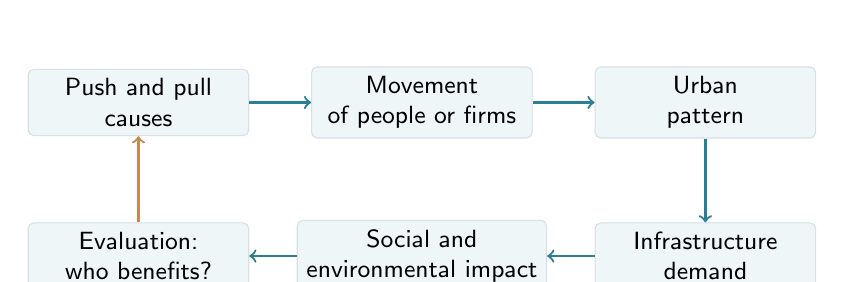
\begin{tikzpicture}[node distance=1.6cm, every node/.style={font=\sffamily\small}]
  \tikzstyle{box}=[rectangle, rounded corners=2pt, draw=RuleGray, fill=SoftBlue,
  minimum width=2.8cm, minimum height=0.8cm, align=center]
  \node[box] (cause) {Push and pull\\causes};
  \node[box, right of=cause, xshift=2.0cm] (move) {Movement\\of people or firms};
  \node[box, right of=move, xshift=2.0cm] (pattern) {Urban\\pattern};
  \node[box, below of=pattern, yshift=-0.35cm] (infra) {Infrastructure\\demand};
  \node[box, left of=infra, xshift=-2.0cm] (impact) {Social and\\environmental impact};
  \node[box, left of=impact, xshift=-2.0cm] (eval) {Evaluation:\\who benefits?};
  \draw[->, thick, color=AccentTeal] (cause) -- (move);
  \draw[->, thick, color=AccentTeal] (move) -- (pattern);
  \draw[->, thick, color=AccentTeal] (pattern) -- (infra);
  \draw[->, thick, color=AccentTeal] (infra) -- (impact);
  \draw[->, thick, color=AccentTeal] (impact) -- (eval);
  \draw[->, thick, color=AccentGold] (eval) -- (cause);
\end{tikzpicture}
\end{center}

\section{Audio 2 Script}
\subsection{Global Climate: Causes, Consequences, Vulnerability, And Resilience}

\textit{Target length: about 12 minutes at a natural revision pace. This script
is for the Paper 2 core unit, so keep stimulus-reading and paragraph precision
in mind while listening.}

Monday, 2026-04-27. Audio 2. \textbf{Minute 0--2: the core frame.}
The second audio moves from Paper 1 Urban environments to the Paper 2 core unit
\term{Global climate - vulnerability and resilience}. The unit is not only
about climate science. It is about how a changing climate creates uneven risk,
why some people and places are more vulnerable, and how societies try to become
more resilient.

Use a four-part frame: \term{cause}, \term{consequence}, \term{vulnerability},
\term{resilience}. Cause asks why the climate is changing. Consequence asks
what changes matter for people and environments. Vulnerability asks who is most
likely to suffer serious harm and why. Resilience asks what capacity exists to
prepare, absorb, recover, and adapt. If you can move through those four steps,
you can organize most climate answers in Paper 2.

\term{Climate change} means long-term change in average conditions and the
frequency or intensity of extremes. Do not confuse it with one day of weather.
\term{Global warming} is the rise in average global temperature, while climate
change includes wider shifts such as changing rainfall, sea-level rise, ice
loss, heatwaves, drought risk, stronger rainfall events, ecosystem shifts, and
ocean warming. In an exam answer, use precise terms rather than saying only "bad
weather."

\textbf{Minute 2--4: causes.}
The central physical process is the \term{enhanced greenhouse effect}. Some
greenhouse gases in the atmosphere absorb outgoing long-wave radiation and help
keep Earth warm enough for life. The problem is that human activity has
increased the concentration of greenhouse gases, strengthening this warming
effect. The main human drivers include burning fossil fuels for electricity,
transport, industry, and heating; deforestation and land-use change; cement and
industrial processes; agriculture; and waste.

Carbon dioxide, or CO$_2$, is strongly linked with fossil-fuel combustion and
deforestation. Methane is linked with livestock, rice cultivation, fossil-fuel
extraction, and waste. Nitrous oxide is linked with fertilizer use and
agriculture. Land-use change matters because forests store carbon and influence
evapotranspiration, surface reflectivity, and local water cycles. When forests
are cleared, stored carbon can be released and future carbon uptake is reduced.

The exam point is not to write a chemistry essay. The exam point is to show
that human energy systems, transport systems, food systems, land use, and
economic development pathways have changed atmospheric composition. This is why
climate change links directly to population, urbanization, food, health, and
resource consumption.

\textbf{Minute 4--7: major consequences.}
Climate consequences can be physical, social, economic, and political. Start
with physical consequences. Higher temperatures can increase heatwave risk and
alter evaporation. Changing rainfall can create drought in some regions and
more intense rainfall or flooding in others. Sea-level rise increases coastal
flooding, erosion, storm-surge impacts, saltwater intrusion, and pressure on
low-lying settlements. Melting glaciers can change seasonal water supply,
especially where rivers depend on meltwater. Ocean warming and acidification
can damage marine ecosystems and fisheries.

Now connect physical consequences to human systems. Food security may be
affected by drought, heat stress, pests, crop failure, lower yields, flooding,
and disrupted transport. Water security may be affected by changing rainfall,
glacier retreat, drought, groundwater stress, contamination after floods, and
competition between households, farms, industry, and energy systems. Health may
be affected by heat stress, malnutrition, water-borne disease after flooding,
vector-borne disease shifts, smoke from fires, mental stress after disasters,
and pressure on healthcare systems.

Settlements and economies can also be affected. Coastal settlements may face
flooding, erosion, expensive protection costs, insurance problems, relocation,
and loss of infrastructure. Urban areas may face heat-island effects, stormwater
flooding, power demand for cooling, and unequal exposure for people in
lower-quality housing. Rural livelihoods may be affected where farming,
pastoralism, fishing, or tourism depends strongly on climate conditions.
Conflict and migration are not automatic outcomes of climate change, but climate
stress can intensify existing poverty, resource insecurity, political weakness,
or social tension.

\textbf{Minute 7--9: vulnerability.}
\term{Vulnerability} means the degree to which people or places are likely to be
harmed by a hazard or long-term stress. It is shaped by \term{exposure},
\term{sensitivity}, and \term{capacity to respond}. Exposure asks whether people
or assets are in harm's way, such as a low-lying coast, drought-prone region, or
floodplain. Sensitivity asks how strongly the system is affected, such as a
farmer relying on rain-fed crops or an elderly person during a heatwave.
Capacity to respond asks whether people have money, infrastructure, governance,
knowledge, insurance, social networks, healthcare, mobility, and political voice.

This is the most important Paper 2 habit: physical hazard is not the same as
human disaster. A cyclone, drought, flood, or heatwave becomes more damaging
when exposed people have fragile housing, weak warning systems, insecure
livelihoods, poor health, limited savings, or little government support. A
wealthy coastal city and a poorer coastal settlement can face similar sea-level
or storm-surge exposure but have very different outcomes because of building
codes, drainage, emergency planning, insurance, and recovery funds.

Vulnerability also varies within one country or city. Older people, children,
outdoor workers, informal-settlement residents, people with disabilities,
low-income households, subsistence farmers, and groups with less political power
may face higher risk. Therefore, a strong answer does not simply say "poor
countries are vulnerable." It explains the mechanism: poverty, housing quality,
livelihood dependence, weak services, and limited recovery capacity increase the
chance that climate stress becomes long-term harm.

\textbf{Minute 9--10: resilience.}
\term{Resilience} is the capacity to prepare for, cope with, recover from, and
adapt to climate stress without collapsing into deeper crisis. It does not mean
no damage. It means damage is reduced, recovery is faster, and future risk is
managed better. Resilience can be built through early-warning systems, stronger
building codes, flood defenses, water storage, drought-resistant crops, social
protection, insurance, public health planning, community networks, ecosystem
restoration, heat-action plans, and more reliable governance.

Separate \term{mitigation} from \term{adaptation}. Mitigation reduces the causes
of climate change, for example by cutting emissions, shifting to renewable
energy, improving efficiency, protecting forests, or changing transport systems.
Adaptation reduces harm from impacts that are already happening or likely to
happen, for example by building flood defenses, changing crop varieties, adding
urban shade, or improving disaster preparation. A resilient place often needs
both. Mitigation without adaptation leaves exposed groups at risk now.
Adaptation without mitigation can become overwhelmed if climate change becomes
more severe.

\textbf{Minute 10--12: model analyse paragraph.}
Here is a model \exam{analyse} paragraph. Climate change creates uneven
consequences because physical exposure interacts with social vulnerability and
resilience. For example, two coastal settlements may both face sea-level rise
and storm-surge risk, but the impact will be greater where housing is informal,
drainage is weak, incomes are low, and warning systems are unreliable. In that
place, flooding can destroy homes, contaminate water, interrupt jobs, and slow
recovery because households have fewer savings or insurance options. By
contrast, a wealthier coastal city with flood defenses, evacuation routes,
building codes, and emergency funds may still suffer damage but recover more
quickly. The consequence of climate change is therefore not determined by the
physical hazard alone; it depends on exposure, sensitivity, and the capacity to
respond.

Notice how that paragraph is analytical rather than only descriptive. It breaks
the issue into parts: hazard, exposure, vulnerability, resilience, and outcome.
It also compares different groups or places. That is what the command term
\exam{analyse} needs. It is not enough to say "climate change causes floods."
You have to show the relationships that turn a physical process into uneven
human impacts.

The student case-study sheet currently has no completed climate case-study
entry. Mark that as a revision gap. Before the exam, fill in at least two
climate anchors: one impact or vulnerability example, and one resilience or
adaptation example. The minimum detail for each is place, hazard, exposed group,
impact, response, and limitation. Until your class notes supply the exact cases,
use general examples carefully and avoid invented statistics.

Pause now and say the four climate words from memory: cause, consequence,
vulnerability, resilience. Then write one chain:
\term{greenhouse gas emissions} $\rightarrow$ \term{physical climate change}
$\rightarrow$ \term{specific hazard} $\rightarrow$ \term{vulnerable group}
$\rightarrow$ \term{impact} $\rightarrow$ \term{resilience or adaptation
response}. That chain will become the second paragraph in the workbook.

\subsection{Climate Key Terms}

\rowcolors{2}{TableStripe}{white}
\begin{tabularx}{\textwidth}{L{0.25\textwidth}Y Y}
\toprule
\textbf{Term} & \textbf{Core meaning} & \textbf{How to use it in an answer} \\
\midrule
Enhanced greenhouse effect & Strengthening of Earth's warming effect because
human activity increases greenhouse gas concentrations & Use for causes:
fossil fuels, land-use change, agriculture, industry, and waste \\
Mitigation & Action to reduce the causes of climate change or greenhouse gas
emissions & Use for emission cuts, renewable energy, efficiency, forest
protection, and transport change \\
Adaptation & Action to reduce harm from climate impacts & Use for flood
defenses, drought planning, crop change, heat-action plans, and water storage \\
Vulnerability & Likelihood of serious harm from a hazard or stress & Explain
through exposure, sensitivity, poverty, infrastructure, governance, and
livelihood dependence \\
Resilience & Capacity to prepare, cope, recover, and adapt & Link to warning
systems, social networks, savings, institutions, infrastructure, and planning \\
Exposure & Presence of people, assets, or systems in places that could be
affected & Use for coasts, floodplains, drylands, heat-prone cities, and
low-lying islands \\
Sensitivity & Degree to which a system is affected by climate stress & Use for
rain-fed farming, elderly populations, poor housing, and fragile ecosystems \\
\bottomrule
\end{tabularx}
\rowcolors{2}{}{}

\subsection{Climate Consequence Matrix}

\rowcolors{2}{TableStripe}{white}
\begin{tabularx}{\textwidth}{L{0.2\textwidth}Y Y}
\toprule
\textbf{System} & \textbf{Possible climate consequence} & \textbf{Vulnerability or resilience angle} \\
\midrule
Food & Crop stress, yield changes, pests, livestock heat stress, disrupted
transport & Rain-fed farmers and low-income consumers are more exposed when
storage, trade, and safety nets are weak \\
Water & Drought, altered rainfall, glacier retreat, flood contamination,
saltwater intrusion & Resilience depends on storage, distribution, pricing,
watershed management, and governance \\
Health & Heat stress, disease risk, malnutrition, disaster injury, mental
stress & Risk rises for elderly people, outdoor workers, children, and
households with weak healthcare access \\
Settlements & Coastal flooding, storm damage, erosion, heat-island effects,
infrastructure loss & Building codes, drainage, insurance, evacuation, and
income strongly affect recovery \\
Ecosystems & Coral stress, species range shifts, wildfire risk, habitat loss &
Protected areas and ecosystem restoration can help but may be limited by rapid
warming or land-use pressure \\
Economies & Infrastructure repair costs, lower productivity, tourism loss,
supply disruption & Diversified economies and stronger institutions usually
recover faster than places dependent on one climate-sensitive sector \\
\bottomrule
\end{tabularx}
\rowcolors{2}{}{}

\section{25-Minute Practice Block}

Use the workbook file \term{2026-04-27-urban-climate-paragraph-workbook.pdf}.
The goal is not to write long essays. The goal is to produce two accurate,
exam-ready paragraphs:

\begin{enumerate}
  \item one \exam{explain} paragraph about urbanization and infrastructure
  pressure
  \item one \exam{analyse} paragraph about climate consequences, vulnerability,
  and resilience
\end{enumerate}

\subsection{Paragraph Rules}

\rowcolors{2}{TableStripe}{white}
\begin{tabularx}{\textwidth}{L{0.17\textwidth}Y Y}
\toprule
\textbf{Command} & \textbf{What the paragraph must do} & \textbf{Common weakness} \\
\midrule
Explain & Give a reason and show how one thing leads to another & Listing
causes without a causal chain \\
Analyse & Break the issue into parts and show relationships between them &
Describing impacts without showing why impacts vary \\
\bottomrule
\end{tabularx}
\rowcolors{2}{}{}

\subsection{End-Of-Day Output}

You are finished with April 27 if you have:

\begin{itemize}
  \item said the difference between centripetal and centrifugal movement from
  memory
  \item written one urbanization-to-infrastructure process chain
  \item explained the enhanced greenhouse effect in two or three accurate
  sentences
  \item listed at least four major climate consequences
  \item used vulnerability and resilience in a climate paragraph
  \item completed and self-marked one \exam{explain} paragraph and one
  \exam{analyse} paragraph
  \item identified one missing climate case-study anchor to fill before
  Thursday 2026-04-30
\end{itemize}

\boxnote{SoftGreen}{Carry forward.}{On Tuesday 2026-04-28, the plan turns to
Food and health plus Resources. Bring forward today's paragraph weakness: if
the issue was causal chains, practise resource-impact chains; if the issue was
case evidence, add exact details to the climate and resources case-study bank.}

\end{document}
